\documentclass[11pt,a4paper]{paper}

\usepackage{preambule}
\fancyhead[L]{\scriptsize \textsc{Nora Nicolas}}

\begin{document}

\title{Referee answer}

\section{Of the surveys' spectroscopic follow-up}
\begin{enumerate}

    \item SNLS's detection efficiency $\e \approx 0$ for $i \approx
        \SI{24.8}{mag}$\smallbreak

        \textcolor{red}{A limiting magnitude of $m_{\lim} = \SI{23.5}{mag}
        \Rightarrow z_{\lim} = 0.36$, which would lead to only 26/236 SNe
    instead of 102/236 with our current cut}
    
    \item HST may have a follow-up efficiency that we should take into account
        like we did for SDSS;

    \item Misunderstanding about the 20\% of SNf's SNe that had selection
        effects:\smallbreak

        \textcolor{dgreen}{The 80\% of SNf's SNe that had no selection
effects are the 114 SNe that are in our sample}.
\end{enumerate}

\section{Of the $x_1$ bias that doesn't appear on $m$}
The referee insists on the fact that ``Biases in x1 are expected as a function
of redshift simply from survey modeling/selection effects'', showing the
following figure from \textsc{Kessler \& Scolnic 2017} to point
out that biases in $x_1$ become apparent much sooner that biases on $m$.

\begin{figure}[htbp!]
    \centering
    \begin{subfigure}[t]{.20\linewidth}
        \centering
        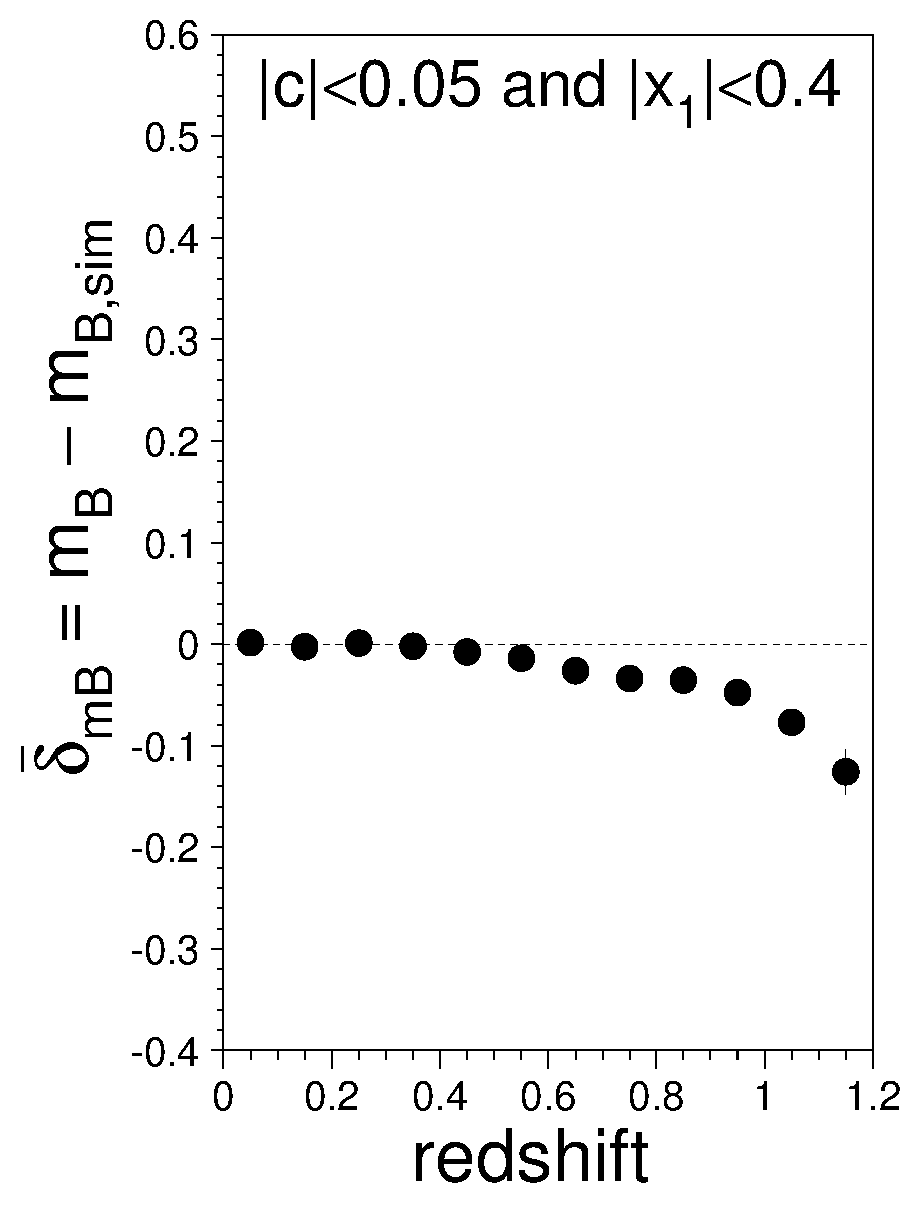
\includegraphics[width=\linewidth]{Answer_figures/Fig_biasCor_mb.eps}
    \end{subfigure}
    \begin{subfigure}[t]{.20\linewidth}
        \centering
        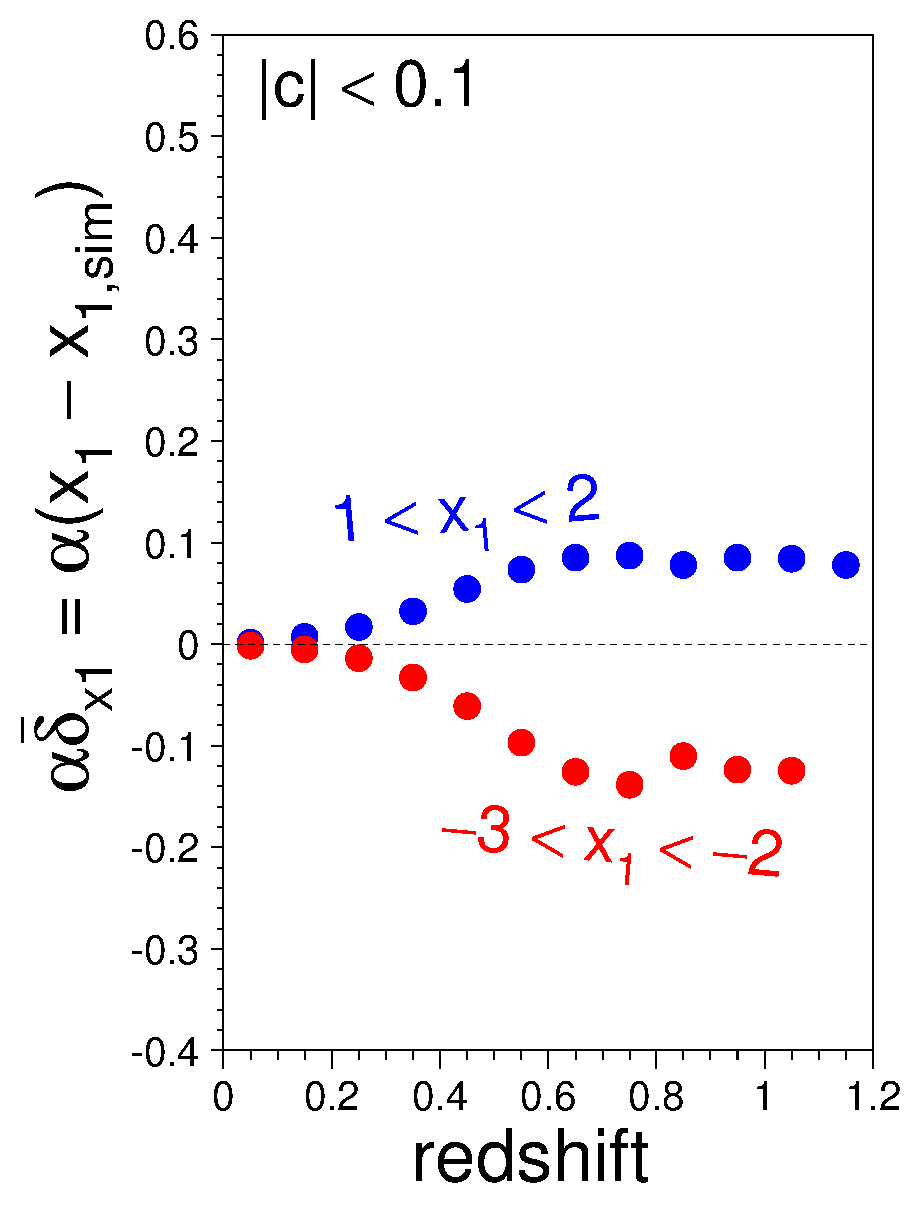
\includegraphics[width=\linewidth]{Answer_figures/Fig_biasCor_x1.eps}
    \end{subfigure}
    \begin{subfigure}[t]{.20\linewidth}
        \centering
        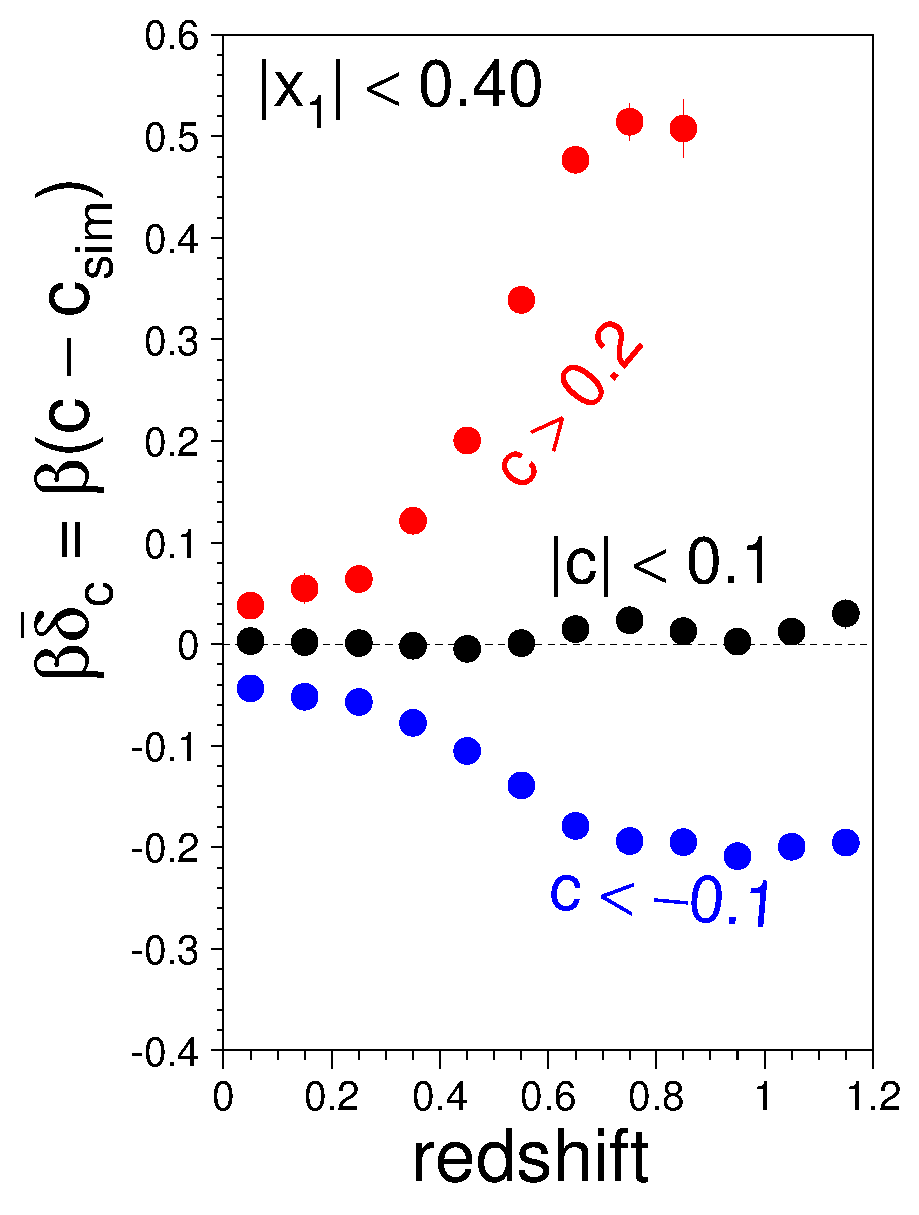
\includegraphics[width=\linewidth]{Answer_figures/Fig_biasCor_c.eps}
    \end{subfigure}
    \captionsetup{justification=centering}
    \caption{Bias corrections $\mkern
        1.5mu\overline{\mkern-1.5mu\delta\mkern-1.5mu}\mkern 1.5mu_{m_B}$,
        $\alpha \overline{\delta}_{x_1}$, and $\beta\overline{\delta}_{c}$ are
        shown as a function of redshift. The pre-factors $\alpha, \beta$ are
        used to show the bias in distance-modulus magnitudes. The parameter
    selection ranges are shown on each panel.}
    \label{fig:KS17}
\end{figure}

\begin{wrapfigure}[13]{R}{.4\linewidth}
    \vspace*{-20pt}
    \centering
    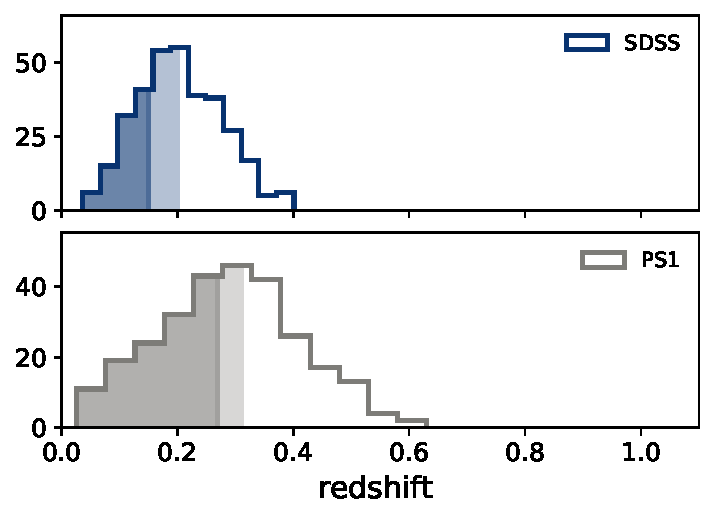
\includegraphics[width=\linewidth]{Answer_figures/hist_surveys2_btw_cividis.pdf}
    \captionsetup{justification=centering}
    \caption{\small Redshift histograms of SNe~Ia from the SDSS and PS1 datasets
    respectively}
    \label{fig:hists}
\end{wrapfigure}
Yet, from the same figure, biases in $c$ appear at $z=0$. Here we want to
convince the referee that if we don't find any sign of color bias in our sample,
we may consider little to no bias on $x_1$. We thus studied the $x_1$ and $c$
distributions of the end of SDSS and the start of PS1, for $0.10 < z < 0.20$. In
this redshift range, the SDSS cut dataset contains the most questionable SNe~Ia,
for the SNe between $0.15 < z < 0.20$ are between our conservative and fiducial
cuts, due to limited spectroscopic resources; the PS1 dataset is however quite
robust for these SNe are far from both the conservative and fiducial cuts; see
Fig. \ref{fig:hists}. \bigbreak

The results are shown Fig. \ref{fig:distrib}. We represented the normed
histograms along with their error bars, and found that they don't differ much.
To ascertain this idea, we used a Kolmogorov-Smirnov test that gave us a p-value
of $0.265$ for the color, and $0.137$ for the stretch; while it doesn't tell us
that both the SDSS and PS1 parts come from the same distribution, as would be
expected if we were free from selection effects (so that the samples were random
draws from what Nature could give us), it is not excluded.

\begin{figure}[htbp!]
    \centering
    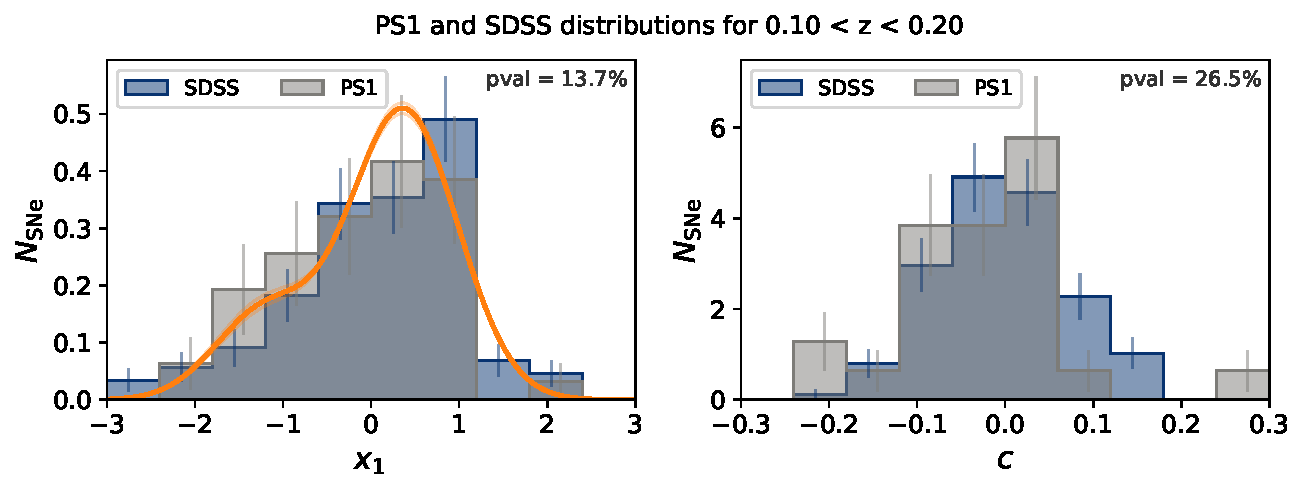
\includegraphics[width=\linewidth]{Answer_figures/both-cut_SDSS_PS1-010-020.pdf}
    \captionsetup{justification=centering}
    \caption{$x_1$ and $c$ normed histograms of the SDSS and PS1 samples for
        $0.10 < z < 0.20$ and their errorbars. On the left, we find in orange
        lines the Base model distributions for $z = 0.10, 0.15, 0.20$ from top
        to bottom. The p-values are the results from a Kolmogorov-Smirnov test;
    they don't show any indication that the samples are not taken from the same
distribution, for both $c$ and $x_1$.}
\label{fig:distrib}
\end{figure}

Moreover, we tried to see if a particular trend of color evolution was visible,
reproducting the Fig. 3 from the original N+20 paper plotting the color instead
of the stretch without any modeling (Fig. \ref{fig:mean_c}), and recalled what
it looked like for the stretch (Fig. \ref{fig:mean_x}). For additional
information, we represented:
\begin{itemize}
    \item The full, uncut dataset in dark grey;
    \item The fiducial sample in light grey;
    \item The SNe above the fiducial cut in green (the SNe that we removed from
        the full sample to obtain the fiducial ones);
    \item The conservative sample il transparent light grey;
    \item And the fiducial sample without HST data.
\end{itemize}
The last one serves to show that even without HST data, the trend of the color
to go up in the last bin is not governed by HST only. We find that the averages
are compatible with a constant mean color, and that the fiducial and
conservative samples are quite close in terms of mean values while removing the
low-color trend that is expected from selection effects. Concerning the stretch,
the fact that the full, fiducial and conservative samples are close are an
indicator that the selection effect have maginal impact on mean $x_1$ in
comparison to the drift.

\begin{figure}[htbp!]
    \centering
    \begin{subfigure}[t]{0.70\linewidth}
        \centering
        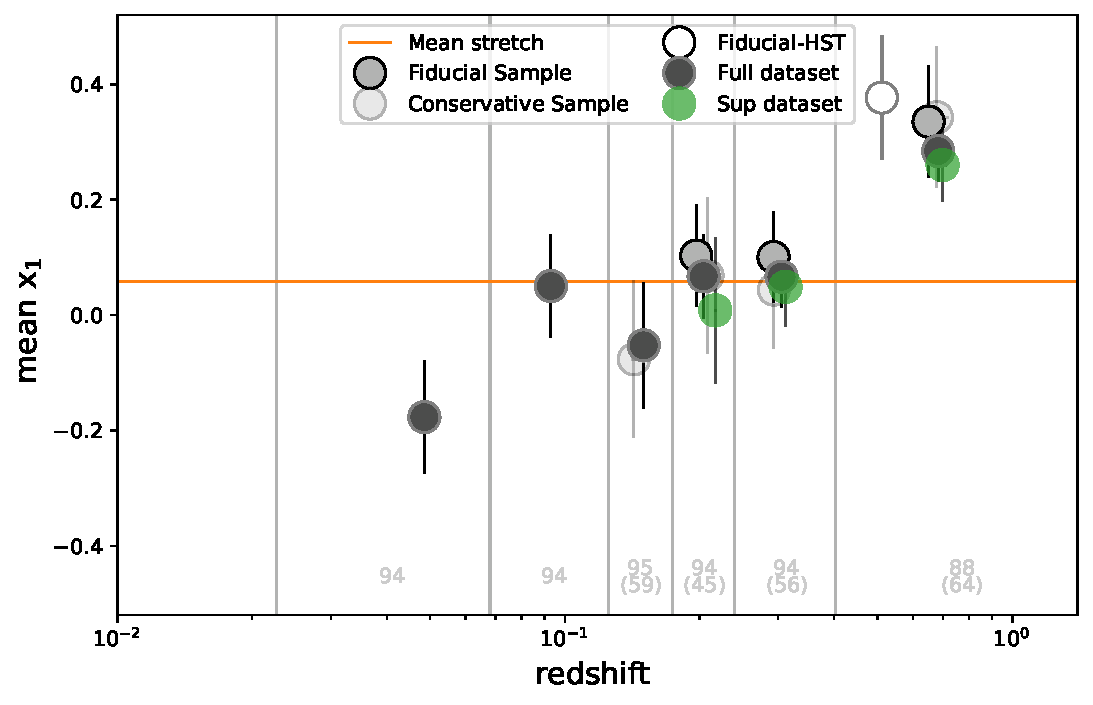
\includegraphics[width=\linewidth]{Answer_figures/mean_stretchs-nHST_full-sup.pdf}
        \captionsetup{justification=centering}
        \caption{Mean stretch of the complete sample}
        \label{fig:mean_x}
    \end{subfigure}
    \begin{subfigure}[t]{0.70\linewidth}
        \centering
        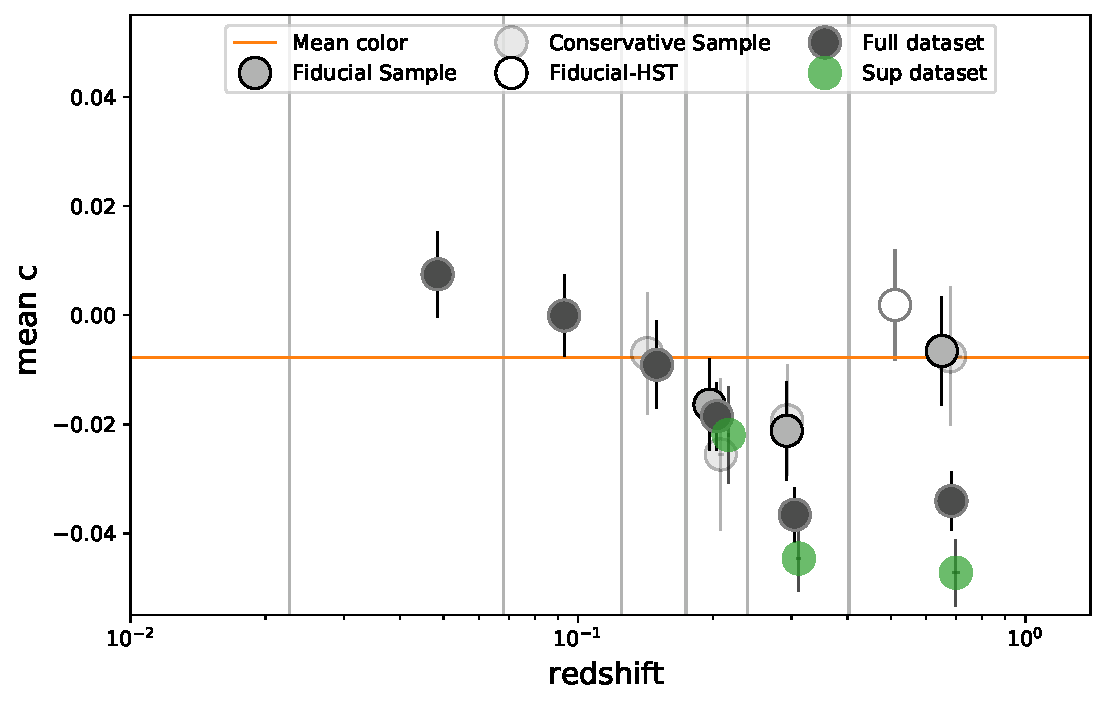
\includegraphics[width=\linewidth]{Answer_figures/mean_colors-nHST_full-sup.pdf}
        \captionsetup{justification=centering}
        \caption{Mean color of the complete sample}
        \label{fig:mean_c}
    \end{subfigure}
    \centering
    \captionsetup{justification=centering}

    \caption{Mean stretch and color of the complete sample in the same 6 bins of
        equal sample size (based on the fiducial sample). The dark grey markers
        represent the full, uncut sample; the light grey ones the fiducial
        sample; the SNe above the fiducial cut are in green; in transparent
        light grey is the conservative sample and the open marker shows the
        means for the complete sample from which we removed HST data. For the
        color, we might think that there is an evolution for the 5 first bins,
        but the 6th one breaks it, even without HST data, while for the stretch,
    with our without HST data we see the same evolution}

    \label{fig:means}
\end{figure}

\section{Of the $x_1$ drift of simulated surveys}
Finally, we wanted to bringto the attention of the referee the fact that a full
SNANA analysis will soon be ongoing and should be the subject of a dedicated
paper, that could then give more in depth insight concerning the simulations
thoughts that were shared with us.
\end{document}
